\subsubsection*{Zadanie~4.}
\begin{mathfigure*}
    \coordinate (A) at (3, 0);
    \coordinate (B) at (0, 4);
    \coordinate (C) at (0, 0);
    \coordinate (M) at (1.5, 2);
    \draw[dashed] (C) -- (M);
    \draw (A) node[below right]{\(A\)}
        -- (B) node[above]{\(B\)}
        -- node[left]{\(4\)} (C) node[below left]{\(C\)}
        -- node[below]{\(3\)} cycle;
    \drawrightangle{A--C--B};
    \path (A) -- node[above right]{\(2{,}5\)} (M) -- node[above right]{\(2{,}5\)} (B);
    \fillpoint*{M}[\(M\)][above right];
\end{mathfigure*}
Z~twierdzenia Pitagorasa mamy \(AB = \sqrt{3^2 + 4^2} = \sqrt{25} = 5\), więc skoro \(M\) jest środkiem odcinka \(AB\), to
\begin{equation*}
    AM = BM = 2{,}5
\end{equation*}
Ponadto, skoro \(CM\) jest środkową trójkąta, to
\begin{equation*}
    \area{AMC} = \area{BMC} = \frac{1}{2}\area{ABC} = \frac{1}{2} \cdot \frac{3 \cdot 4}{2} = 3
\end{equation*}
Wiemy, że
\begin{gather*}
    3 = \area{AMC} = \frac{r_1\pars{AM + MC + CA}}{2}
        = \frac{r_1\pars{2{,}5 + MC + 3}}{2}
        \implies r_1 = \frac{6}{5{,}5 + MC}\\
    3 = \area{BMC} = \frac{r_2\pars{BM + MC + CB}}{2}
        = \frac{r_2\pars{2{,}5 + MC + 4}}{2}
        \implies r_2 = \frac{6}{6{,}5 + MC}
\end{gather*}
Wystarczy zatem obliczyć długość \(MC\). Można to zrobić łatwo przez umieszczenie trójkąta w~układzie współrzędnych w~taki sposób, że
\begin{gather*}
    C = \seq{0; 0}\\
    A = \seq{3; 0}\\
    B = \seq{0; 4}
\end{gather*}
Widzimy, że wtedy \(M = \seq{\frac{3}{2}, 2}\), więc
\begin{equation*}
    CM = \sqrt{1{,}5^2 + 2^2}
        = \sqrt{2{,}25 + 4}
        = \sqrt{6{,}25}
        = 2{,}5
\end{equation*}
Zatem
\begin{gather*}
    r_1 = \frac{6}{5{,}5 + 2{,}5}
        = \frac{6}{8}
        = \frac{3}{4}\\
    r_2 = \frac{6}{6{,}5 + 2{,}5}
        = \frac{6}{9}
        = \frac{2}{3}\\
    r_1 - r_2 = \frac{9}{12} - \frac{8}{12}
        = \frac{1}{12}
\end{gather*}
\subsubsection*{Zadanie~5.}
\begin{mathfigure*}
    \coordinate (X) at (-3, 0);
    \coordinate (Y) at (3, 0);
    \coordinate (Z) at (1, 2.3);
    \coordinate (W) at (-1, 2.3);
    \coordinate (H) at (-1, 0);
    \drawrightangle{W--H--X};
    \draw (X) node[below left]{\(X\)}
        -- node[below]{\(a\)} (Y) node[below right]{\(Y\)}
        -- node[above right]{\(c\)} (Z) node[above right]{\(Z\)}
        -- node[above]{\(b\)} (W) node[above left]{\(W\)}
        -- node[above left]{\(c\)} cycle;
    \draw[dashed] (W) -- node[right]{\(h\)} (H) node[below]{\(H\)};
\end{mathfigure*}
Skoro trapez jest cykliczny, to jest równoramienny. Natomiast jeśli da się w~niego wpisać okrąg, to sumy długości par przeciwległych boków są równe:
\begin{gather*}
    a + b = c + c\\
    c = \frac{a + b}{2}
\end{gather*}
Z~twierdzenia Pitagorasa w~\(\triangle{XHW}\) mamy
\begin{gather*}
    h^2 = c^2 - XH^2\\
    XH = \frac{a - b}{2}\\
    h^2 = c^2 - XH^2
        = \pars{\frac{a + b}{2}}^2 - \pars{\frac{a - b}{2}}^2
        = \frac{4ab}{4}
        = ab\\
    h = \sqrt{ab}\\
    \area{XYZW} = \frac{\pars{a + b}h}{2}
        = \frac{\pars{a + b}\sqrt{ab}}{2}
\end{gather*}
\subsubsection*{Zadanie~6.}
\begin{mathfigure*}
    \coordinate (A) at (0, 0);
    \coordinate (B) at (6, 0);
    \coordinate (C) at (0, 2.5);
    \coordinate (I) at (1, 1);
    \coordinate (r1) at (0, 1);
    \coordinate (r2) at (1, 0);
    \coordinate (O) at (3, 1.25);
    \drawrightangle[angle radius=0.3cm]{B--A--C};
    \draw[ForestGreen, dashed] (I) -- node[above]{\(r\)} (r1);
    \draw[ForestGreen, dashed] (I) -- node[right]{\(r\)} (r2);
    \draw[ForestGreen] (I) circle[radius=1];
    \draw (A)
        -- node[below]{\(a\)} (B)
        -- node[above right]{\(c\)} (C)
        -- node[right, near start]{\(b\)} cycle;
    \draw[RoyalBlue, thick] (O) circle[radius=3.25];
    \draw[RoyalBlue, very thick, dashed] (O) -- node[above, sloped]{\(R\)} (B);
    \fillpoint*[1][ForestGreen][ForestGreen]{I}[\(I\)][above right];
    \fillpoint*[1][RoyalBlue][RoyalBlue]{O}[\(O\)][below left];
\end{mathfigure*}
\begin{gather*}
    r = \frac{a + b - c}{2}\\
    2r = a + b - c\\
    R = \frac{c}{2}\\
    4R = 2c\\
    \textrm{Obw.} = a + b + c = a + b - c + 2c = 2r + 4R
\end{gather*}
\subsubsection*{Zadanie~7.}
Bez straty ogólności zakładamy, że \(k \geq 1\). W~innym przypadku po prostu rozpatrujemy podstawy odwrotnie.
\begin{figure}[H]
    \centering
    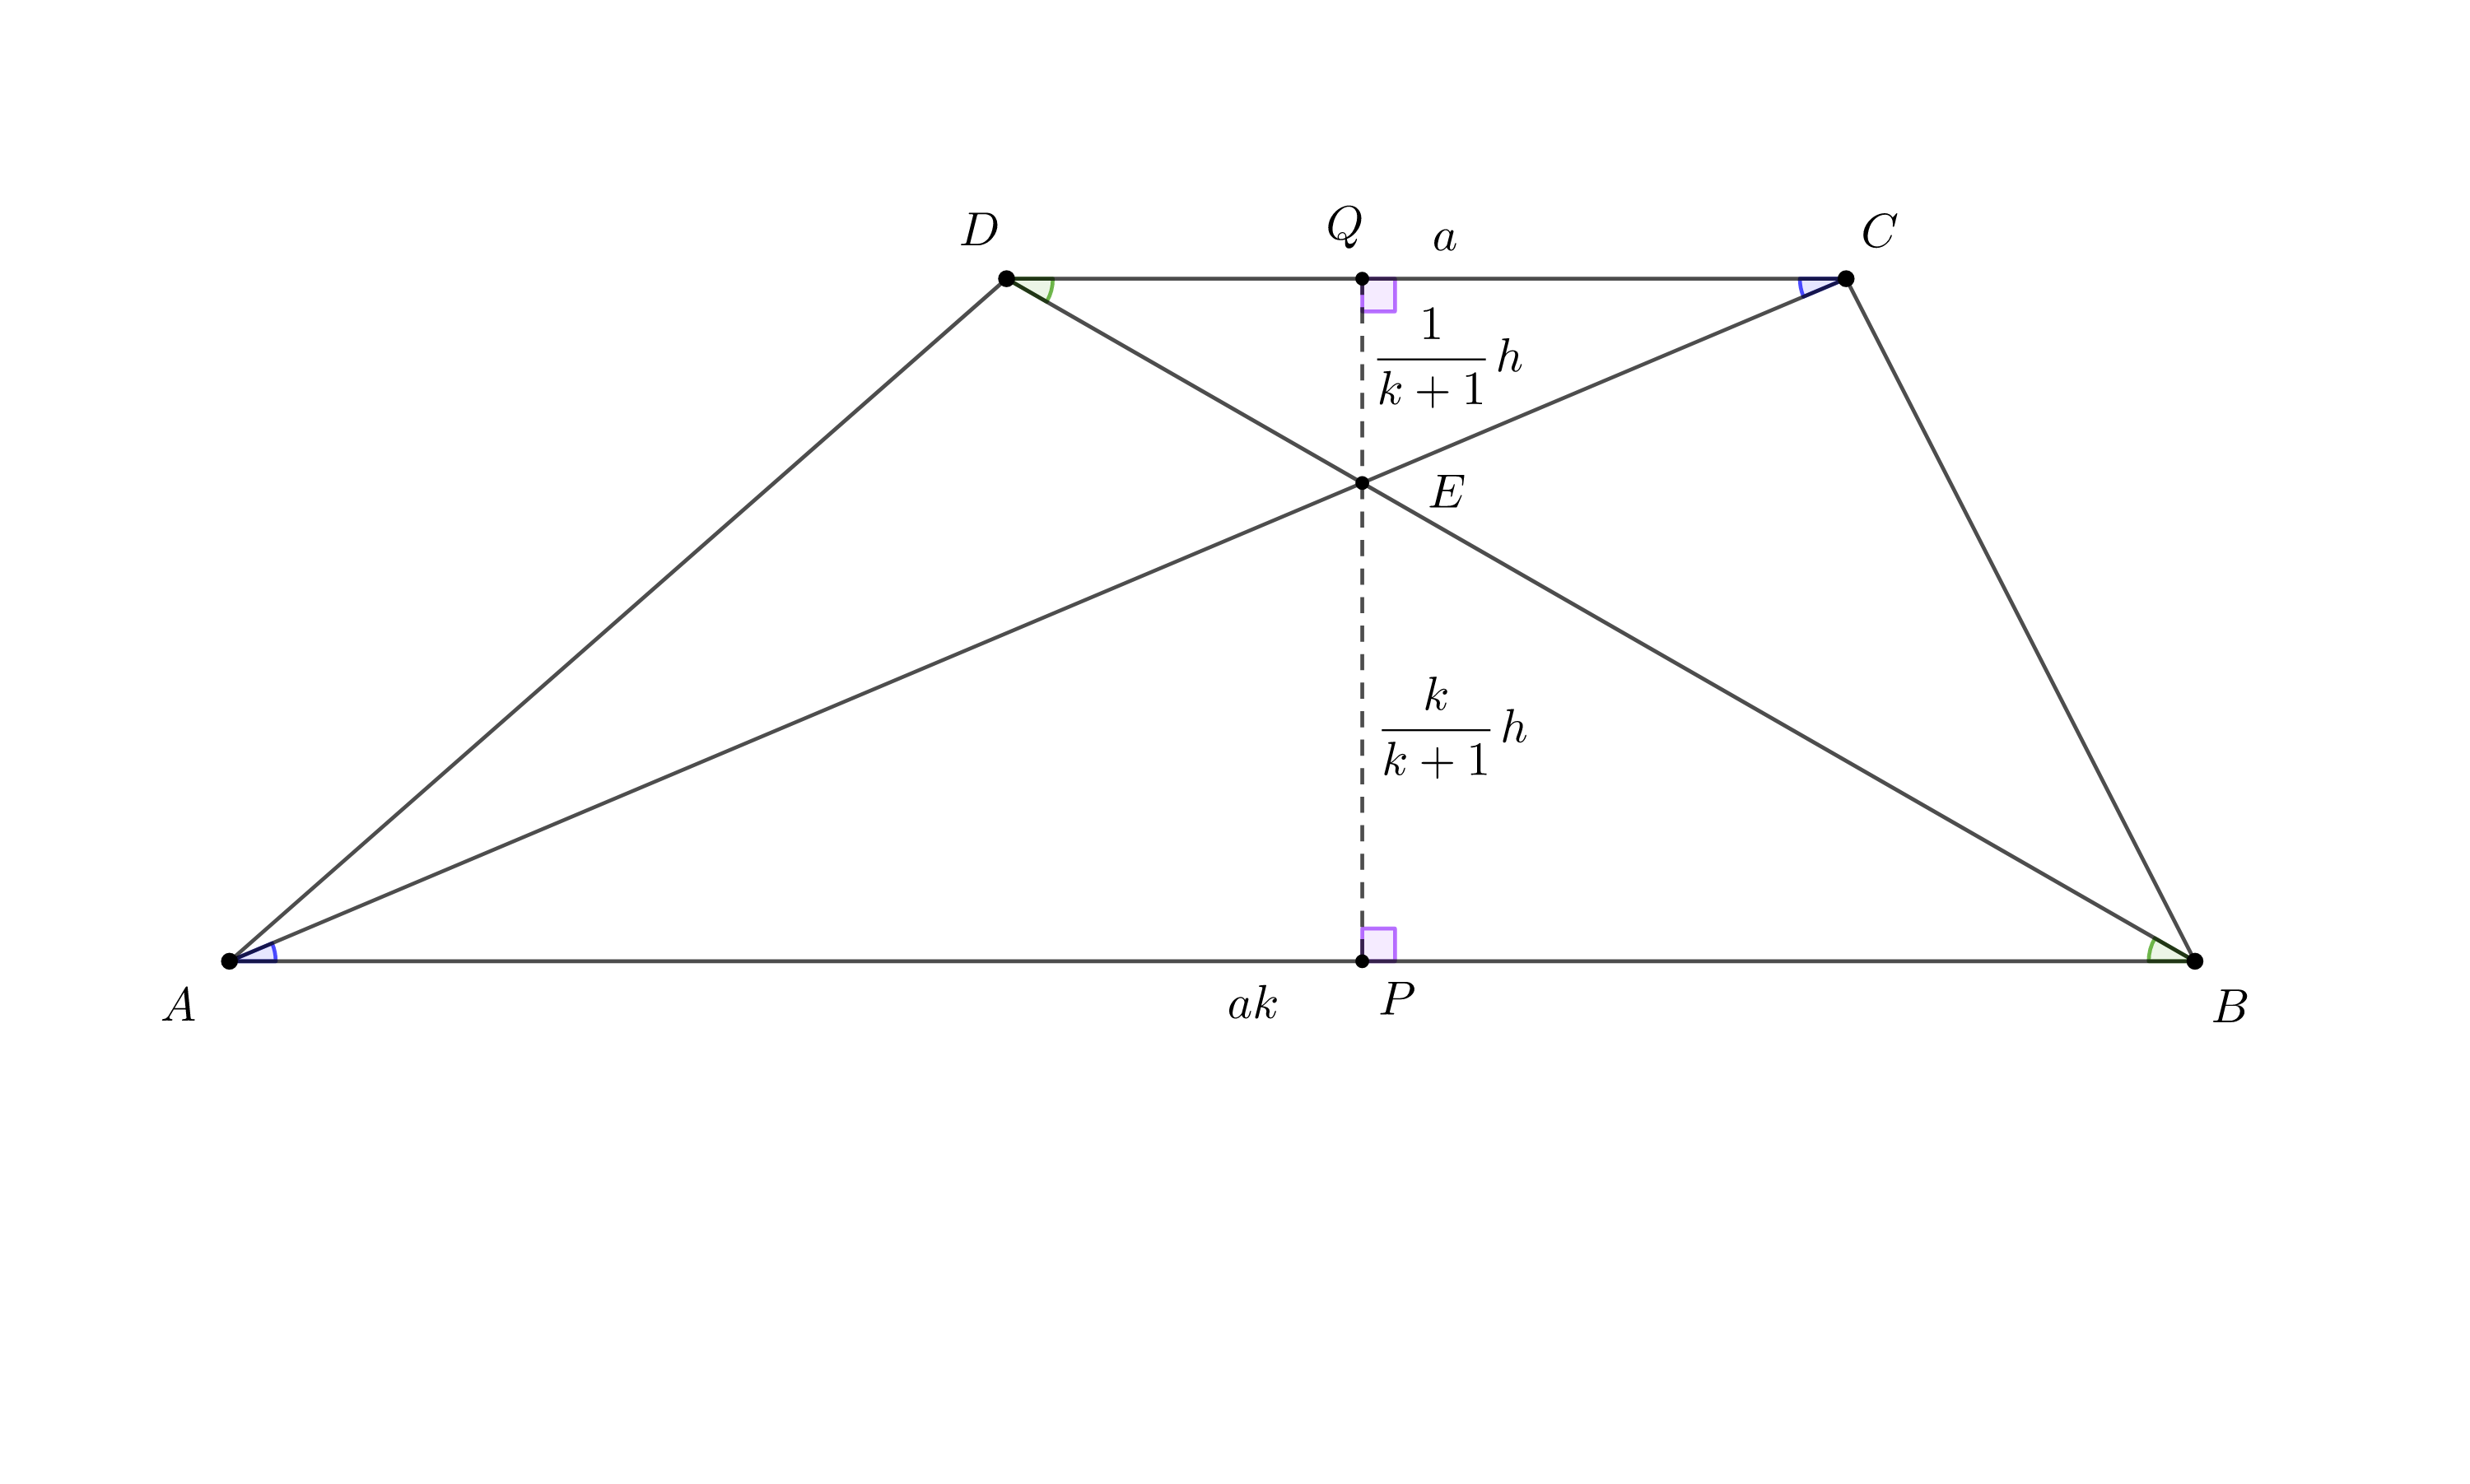
\includegraphics[width=0.8\textwidth]{img/2020_12_16/7.png}
\end{figure}
\begin{gather*}
    \triangle{ABE} \sim \triangle{CED} \implies \frac{PE}{QE} = \frac{AB}{CD} = k\\
    PE = k \cdot QE\\
    h = PE + QE = k \cdot QE + QE = QE \cdot \pars{k + 1}\\
    S = \frac{\pars{ak + a}h}{2} = \frac{ah\pars{k + 1}}{2}\\
    \area{ABE} = \frac{AB \cdot PE}{2}
        = \frac{ak \cdot \frac{k}{k + 1}h}{2}
        = \frac{ahk \cdot \frac{k}{k + 1}}{2}
        = \frac{ah\pars{k + 1} \cdot \frac{k}{k + 1} \cdot \frac{k}{k + 1}}{2}
        = S \cdot \pars{\frac{k}{k + 1}}^2\\
    \area{CDE} = \frac{1}{k^2} \cdot \area{ABE} = S \cdot \pars{\frac{1}{k + 1}}^2\\
    \begin{split}
        \area{BEC} &= \area{ABC} - \area{ABE}
            = \frac{ak \cdot h}{2} - S \cdot \pars{\frac{k}{k + 1}}^2
            = \frac{ah\pars{k + 1} \cdot \frac{k}{k + 1}}{2} - S \cdot \pars{\frac{k}{k + 1}}^2\\
            &= S \cdot \frac{k}{k + 1} - S \cdot \pars{\frac{k}{k + 1}}^2
            = S \cdot \frac{k}{k + 1} \cdot \pars{1 - \frac{k}{k + 1}}
    \end{split}\\
    \begin{split}
        \area{DEA} &= \area{CDA} - \area{CDE}
            = \frac{ah}{2} - S \cdot \pars{\frac{1}{k + 1}}^2
            = \frac{ah\pars{k + 1} \cdot \frac{1}{k + 1}}{2} - S \cdot \pars{\frac{1}{k + 1}}^2\\
            &= S \cdot \frac{1}{k + 1} - S \cdot\pars{\frac{1}{k + 1}}^2
            = S \cdot \frac{1}{k + 1} \cdot \pars{1 - \frac{1}{k + 1}}
    \end{split}
\end{gather*}
\subsubsection*{Zadanie~8.}
\begin{figure}[H]
    \centering
    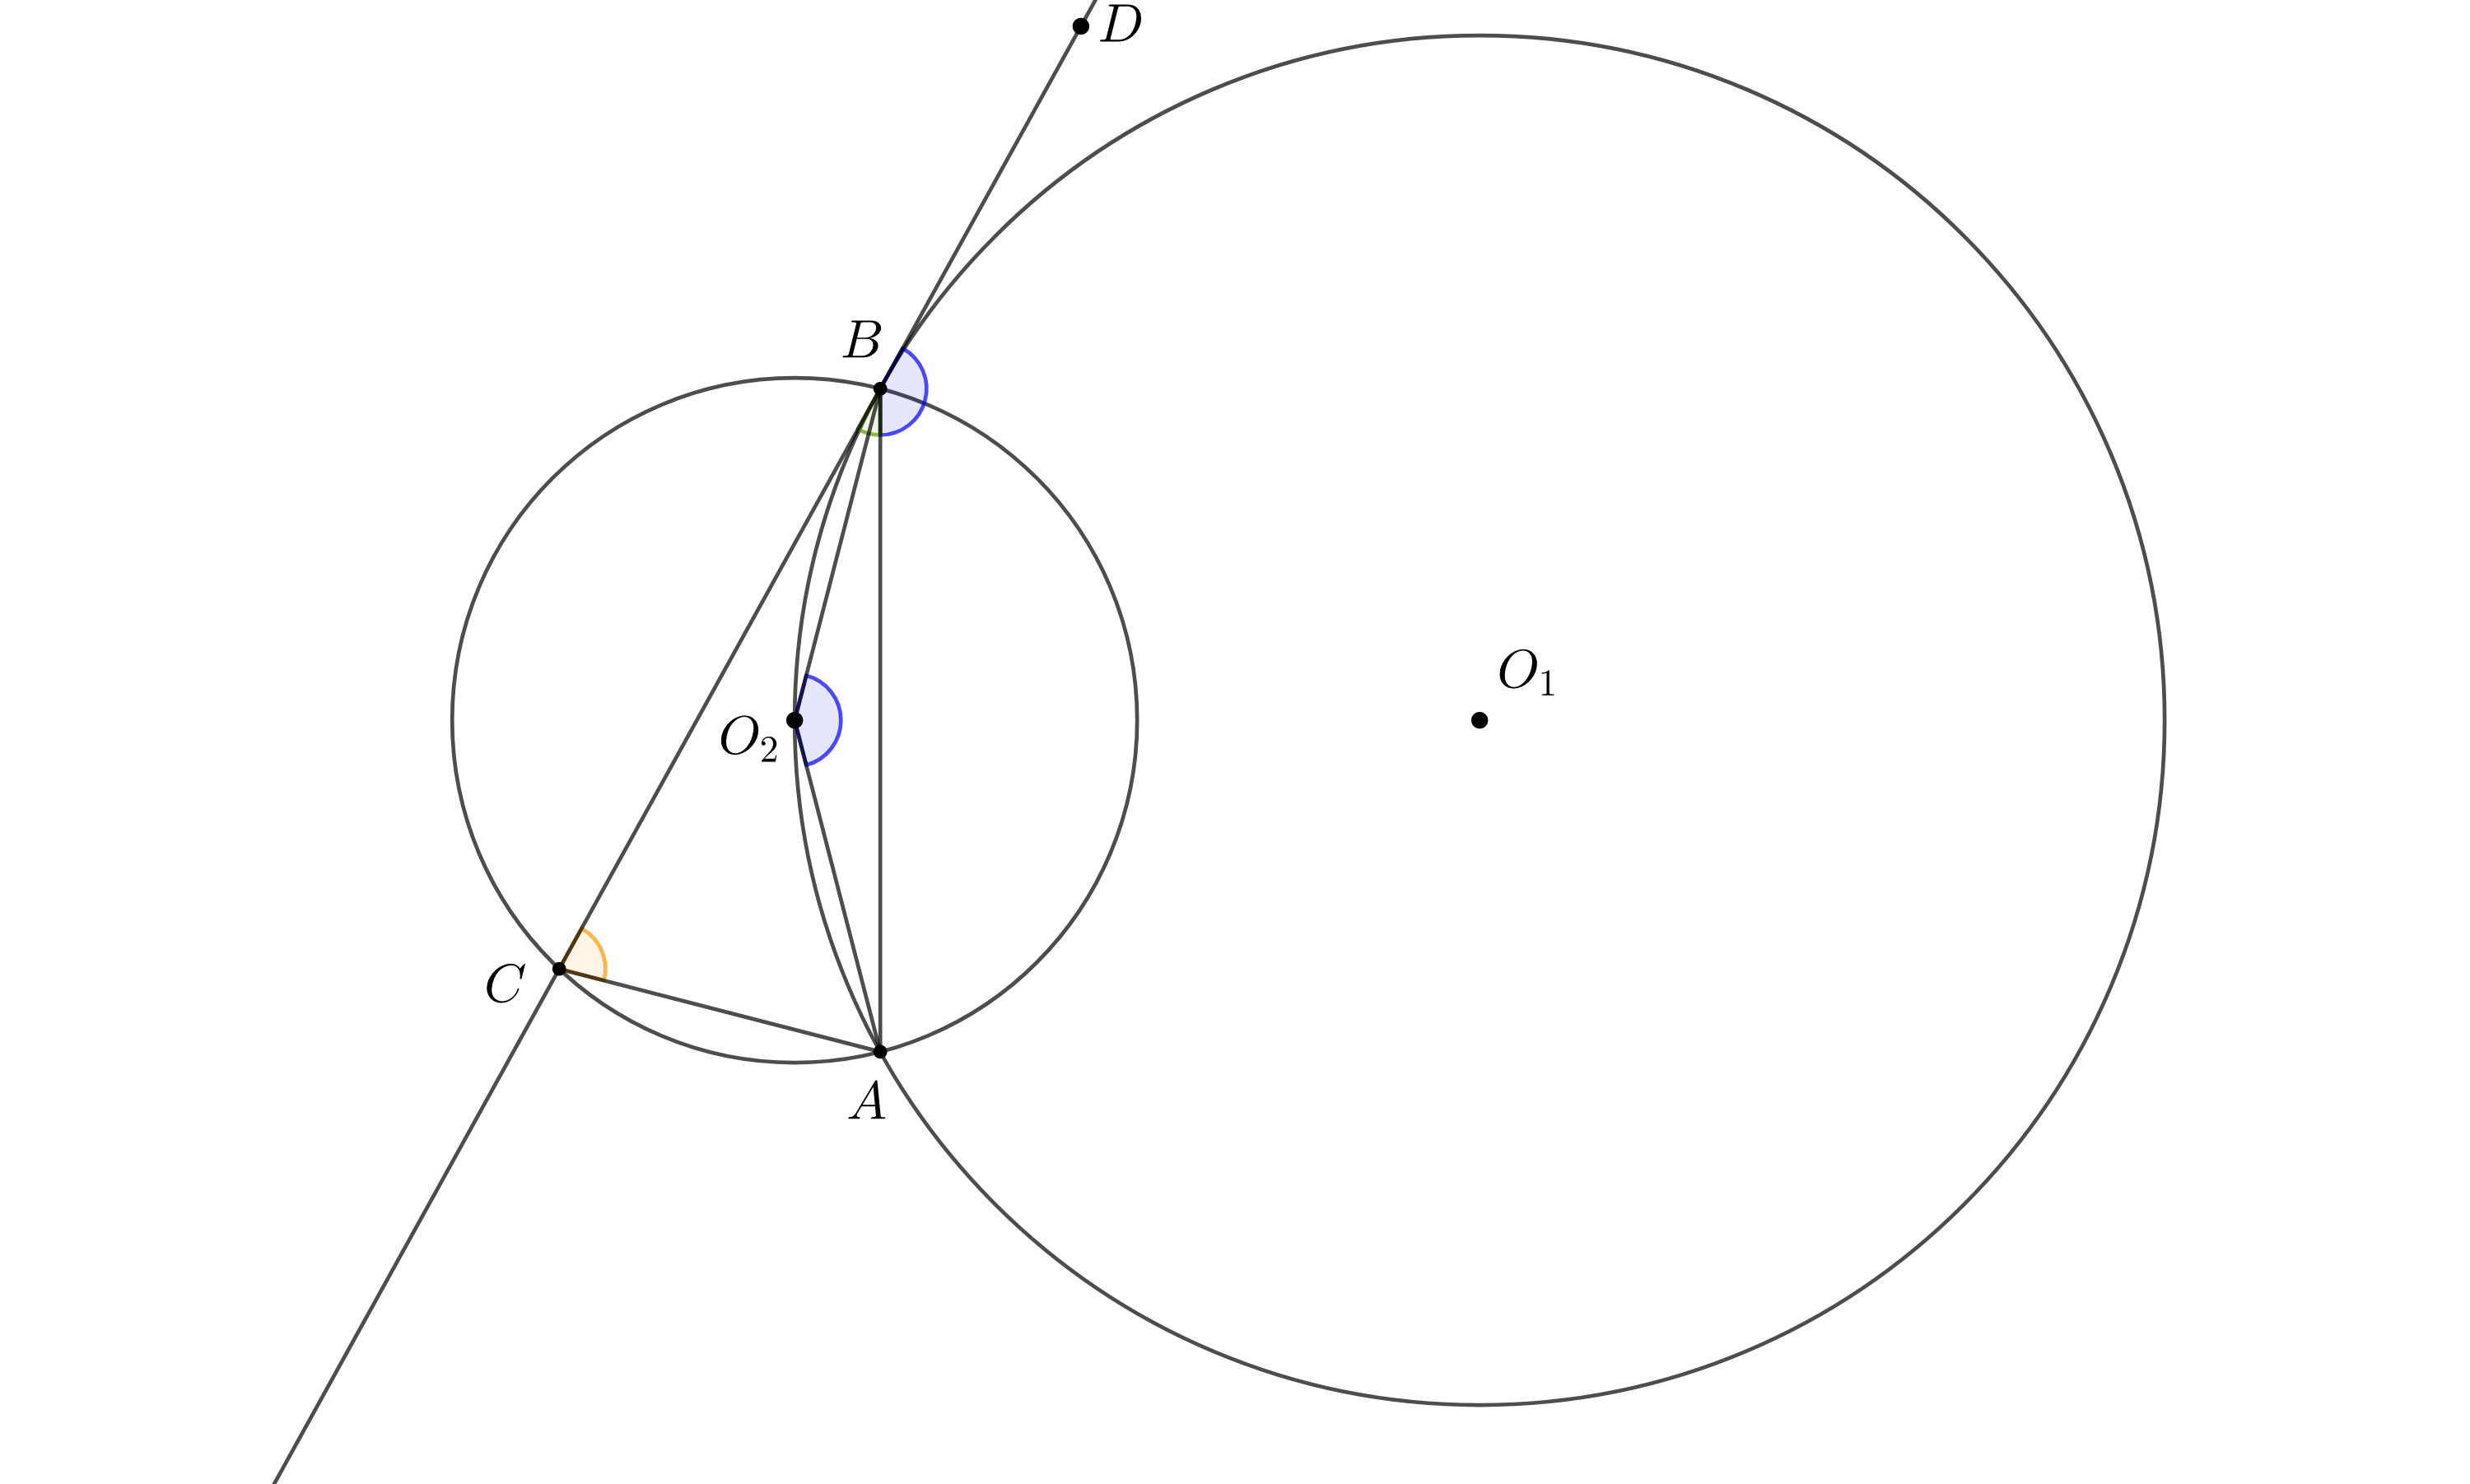
\includegraphics[width=0.8\textwidth]{img/2020_12_16/8.png}
\end{figure}
Ponieważ prosta \(BC\) jest styczna do~okręgu \(O_1\), to z~twierdzenia o~kącie między styczną i~cięciwą:
\begin{equation*}
    \mangle{DBA} = \mangle{BO_2A}
\end{equation*}
Oznaczmy tę wspólną miarę kąta przez \(\alpha\). Ponieważ kąt \(\angle{BCA}\) jest wpisany oparty na tym samym łuku co kąt środkowy \(\mangle{BO_2A} = \alpha\), to \(\mangle{BCA} = \frac{\alpha}{2}\). Z~kątów przyległych mamy:
\begin{equation*}
    \mangle{ABC} = 180\degree - \mangle{DBA} = 180\degree - \alpha
\end{equation*}
Z~sumy kątów w~\(\triangle{ABC}\) mamy więc:
\begin{equation*}
    \mangle{BAC} = 180\degree - \mangle{BCA} - \mangle{ABC}
        = 180\degree - \frac{\alpha}{2} - \pars{180\degree - \alpha}
        = \frac{\alpha}{2}
        = \mangle{BCA}
\end{equation*}
Zatem \(\triangle{ABC}\) jest równoramienny, więc \(AB = BC\).
\qed
\subsubsection*{Zadanie~10.}
\begin{figure}[H]
    \centering
    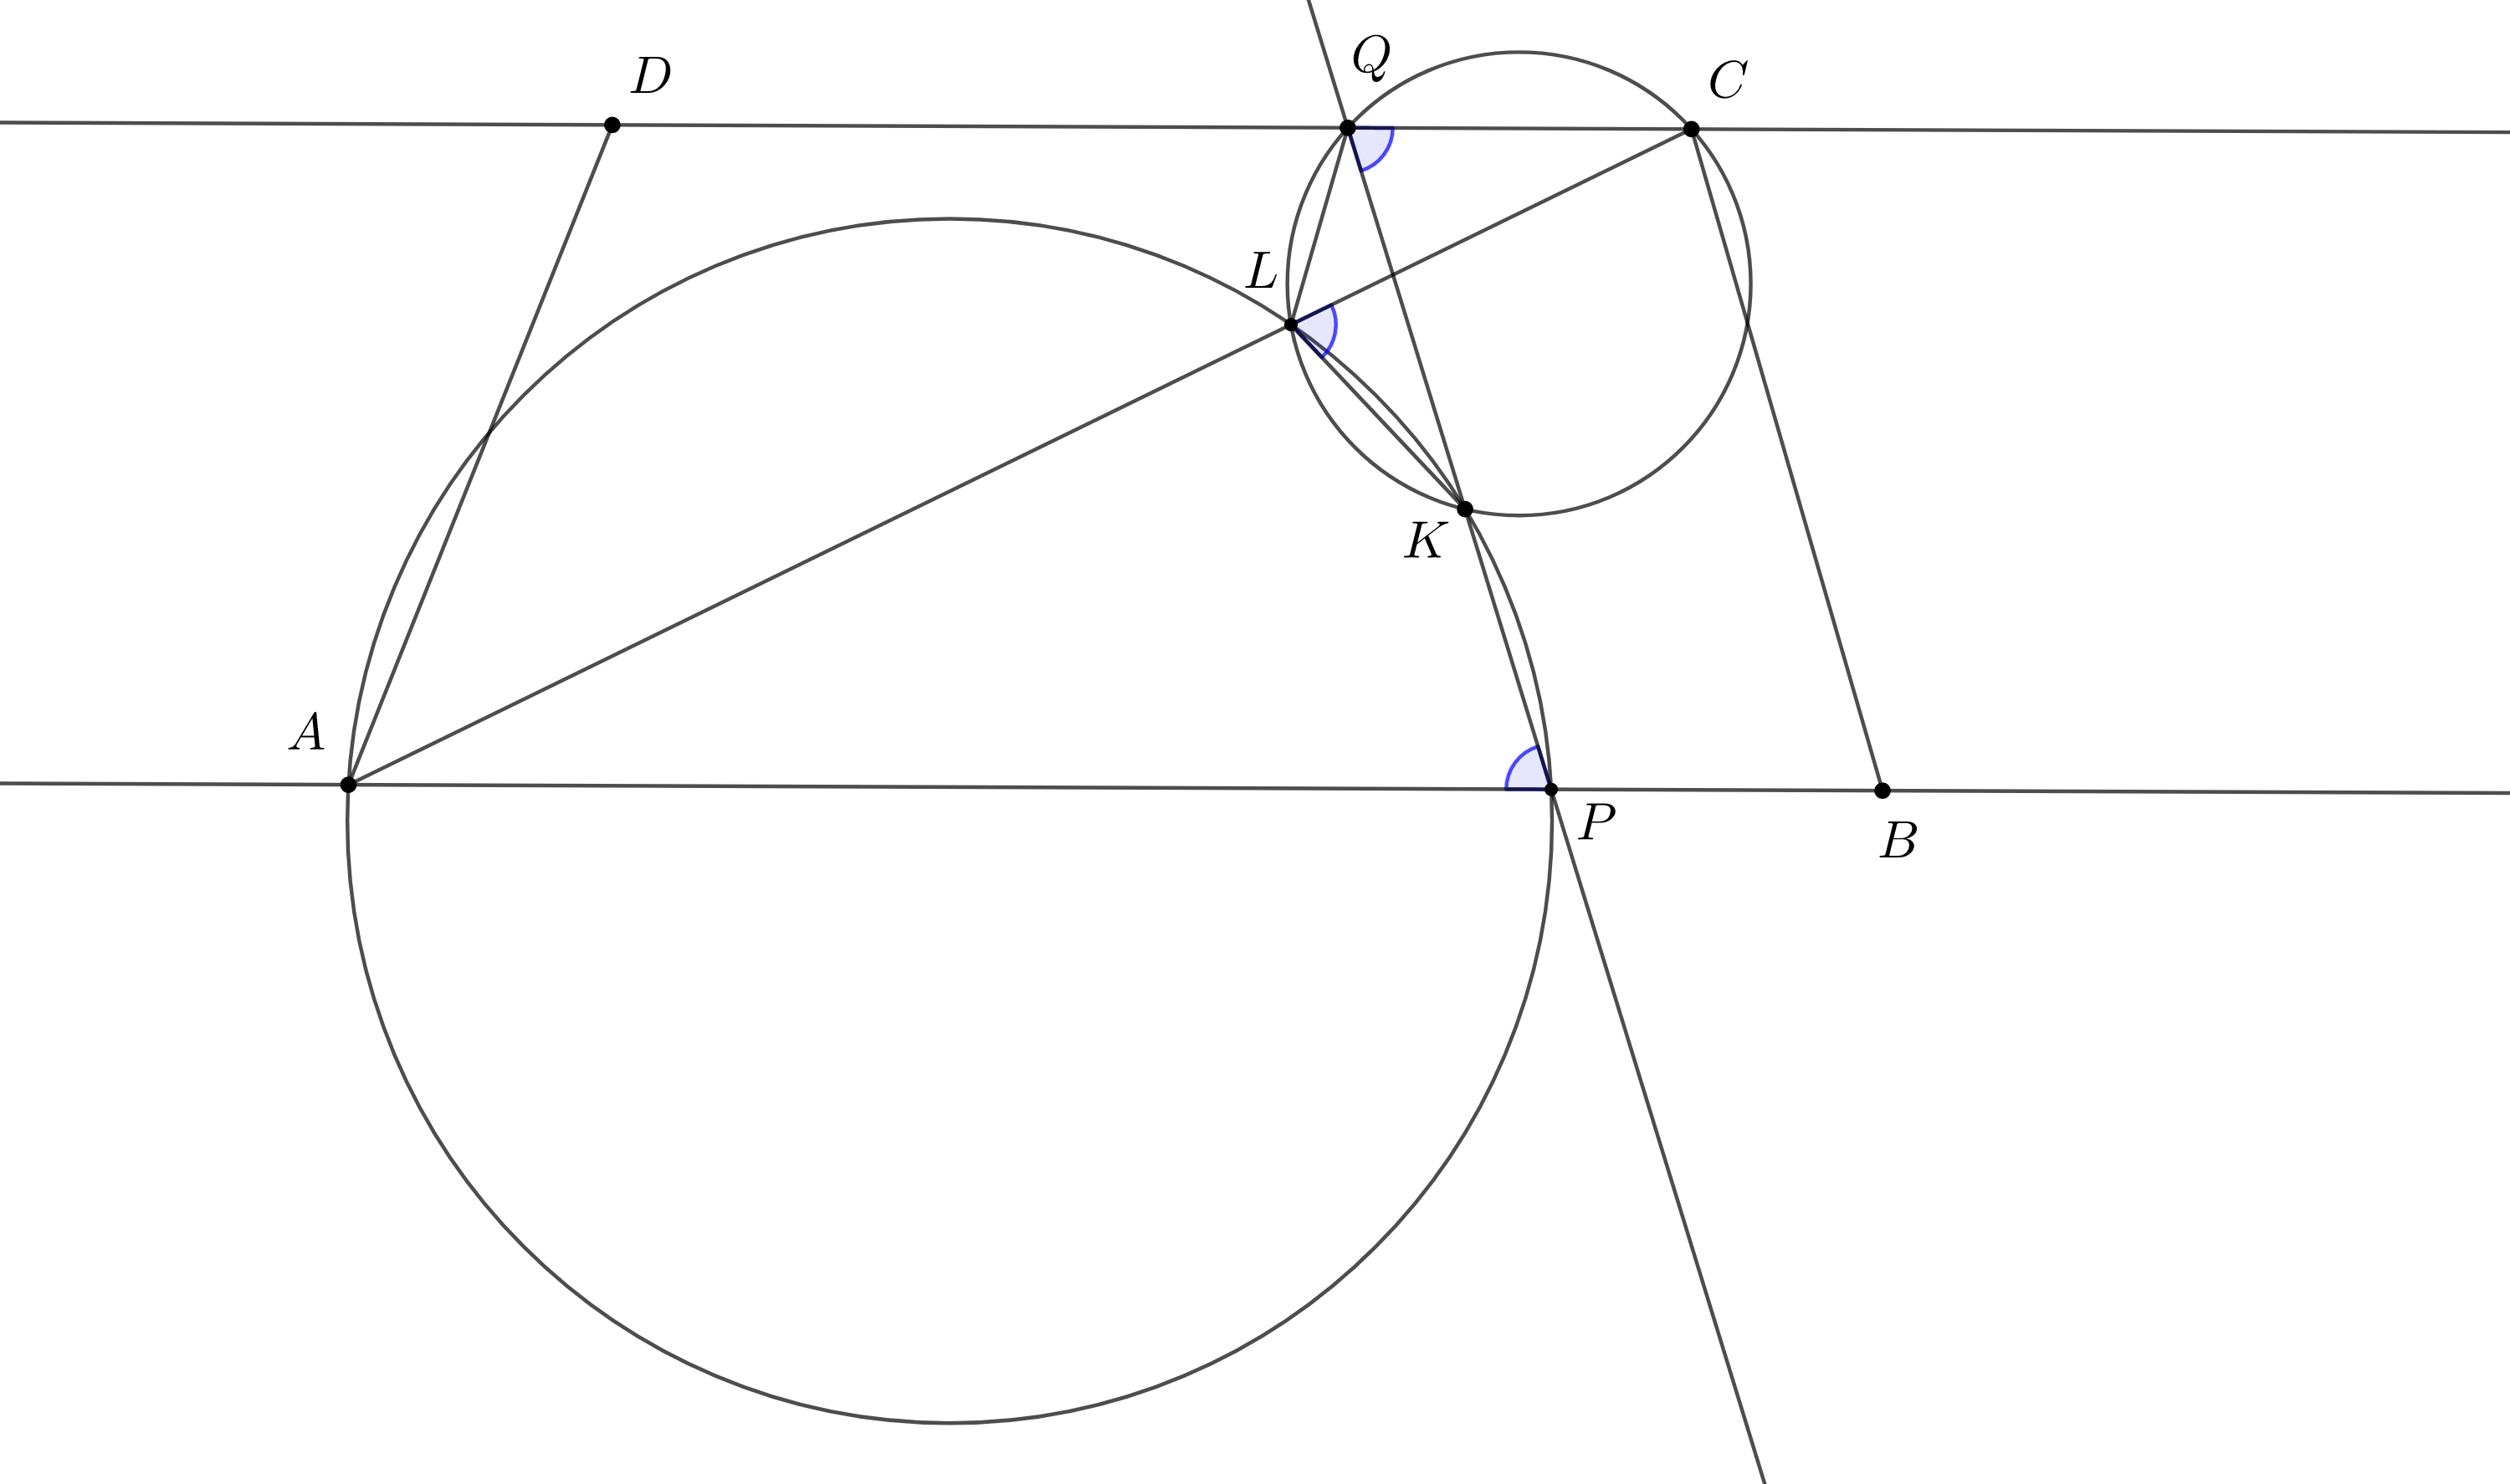
\includegraphics[width=0.8\textwidth]{img/2020_12_16/10.png}
\end{figure}
Przyjmijmy, że \(\mangle{KLC} = \alpha\). Ponieważ \(\angle{KLC}\) i~\(\angle{KQC}\) są oparte na tym samym łuku, to również \(\mangle{KQC} = \alpha\). Skoro czworokąt \(ABCD\) jest trapezem, to \(AB \parallel CD\), więc \(\mangle{KPA} = \mangle{KQC} = \alpha\). Czworokąt \(APKL\) jest wpisany w~okrąg, zatem \(\mangle{KLA} = 180\degree - \mangle{KPA} = 180\degree - \alpha\). Mamy więc
\begin{equation*}
    \mangle{ALC}
        = \mangle{KLA} + \mangle{KLC}
        = 180\degree - \alpha + \alpha
        = 180\degree
\end{equation*}
Zatem \(L\) leży na \(AC\). W~konfiguracji, gdy \(K\) leży po drugiej stronie \(AC\), za \(\alpha\) przyjmujemy miarę kąta \(\angle{KLA}\) i~dowód przebiega analogicznie.
\qed
